\documentclass[12pt, a4paper]{report}

\usepackage{amsmath,amsthm,amssymb}
\usepackage{mathtext}
\usepackage[T1,T2A]{fontenc}
\usepackage[utf8]{inputenc}
\usepackage[english,russian]{babel}
\usepackage{listings}
\usepackage{graphicx}
\usepackage{indentfirst}
\usepackage{float}
\usepackage{tablefootnote}
\usepackage{color}
\usepackage{caption}
\captionsetup[table]{singlelinecheck=off}
\captionsetup[lstlisting]{singlelinecheck=off, labelformat=empty}
\usepackage{pgfplots}
\pgfplotsset{compat=1.9}
\usepackage[left=3cm,right=1cm, top=2cm,bottom=2cm,bindingoffset=0cm]{geometry}
\graphicspath{{./img/}}

\lstset{ 
  backgroundcolor=\color{white},   % choose the background color; you must add \usepackage{color} or \usepackage{xcolor}; should come as last argument
  breaklines=true,                 % sets automatic line breaking
  captionpos=t,                    % sets the caption-position to bottom
  commentstyle=\color{green},    % comment style
  keywordstyle=\color{blue},       % keyword style
  language=Python,                 % the language of the code
  numbers=left,                    % where to put the line-numbers; possible values are (none, left, right)
  numbersep=5pt,                   % how far the line-numbers are from the code
  numberstyle=\tiny\color{black}, % the style that is used for the line-numbers
  showspaces=false,                % show spaces everywhere adding particular underscores; it overrides 'showstringspaces'
  showstringspaces=false,          % underline spaces within strings only
  showtabs=false,                  % show tabs within strings adding particular underscores
  stepnumber=1,                    % the step between two line-numbers. If it's 1, each line will be numbered
  stringstyle=\color{yellow},     % string literal style
  tabsize=2,	                   % sets default tabsize to 2 spaces
  frame=single
}

\begin{document}

\begin{titlepage}
	\noindent \begin{minipage}{0.15\textwidth}
	
\includegraphics[width=\linewidth]{bauman_image}
	\end{minipage}
	\footnotesize\noindent \begin{minipage}{0.8\textwidth}\centering
		\textbf{Министерство науки и высшего образования Российской Федерации}\\
		\textbf{Федеральное государственное бюджетное образовательное учреждение}\\
		\textbf{высшего образования}\\
		\textbf{~~~«Московский государственный технический университет}\\
		\textbf{имени Н.Э.~Баумана}\\
		\textbf{(национальный исследовательский университет)»}\\
		\textbf{(МГТУ им. Н.Э.~Баумана)}
	\end{minipage}
	
	\noindent\rule{17cm}{3pt}
	\newline\newline
	\large\noindent ФАКУЛЬТЕТ $\underline{\text{Информатика и системы управления}}$ \newline\newline
	\noindent КАФЕДРА $\underline{\text{Программное обеспечение ЭВМ и информационные технологии}}$\newline\newline\newline\newline\newline
	
	
	\begin{center}
		\noindent
			\LARGE\textbf{Отчёт по лабораторной работе №1}\newline
			\textbf{по дисциплине "Анализ алгоритмов"}\newline\newline
	\end{center}
	
	\large\noindent\textbf{Тема} $\underline{\text{Расстояние Левенштейна}}$\newline\newline
	\noindent\textbf{Студент} $\underline{\text{Жабин Д.В.}}$\newline\newline
	\noindent\textbf{Группа} $\underline{\text{ИУ7-54Б}}$\newline\newline
	\noindent\textbf{Преподаватель} $\underline{\text{Волкова Л.Л.}}$\newline\newline\newline
	
	\begin{center}
		\large\vfill
		Москва, 2021 г.
	\end{center}
\end{titlepage}

\setlength{\parindent}{1.25cm}

\setcounter{page}{2}\large\linespread{1.3}\tableofcontents

\newpage
\chapter*{Введение}
\addcontentsline{toc}{chapter}{Введение}

\textbf{Расстояние Левенштейна} [1] — метрика, измеряющая по модулю разность между двумя последовательностями символов. Она определяется как минимальное количество односимвольных операций (а именно вставки, удаления, замены), необходимых для превращения одной последовательности символов в другую.
\newline

Расстояние Левенштейна применяется в теории информации и компьютерной лингвистике для:

\begin{itemize}
	\item поиска опечаток в запросах поисковых систем;
	\item автоисправления ошибок в словах;
	\item сравнения текстовых файлов утилитой diff;
	\item сравнения генов, хромосом и белков в биоинформатике.
\end{itemize}

Целью данной работы является исследование различных вариаций алгоритмов нахождения расстояния Левенштейна и Дамерау-Левенштейна.

Для достижения поставленной цели необходимо решить следующие задачи:
\begin{itemize}
  	\item изучить и реализовать алгоритмы Левенштейна и Дамерау-Левенштейна;
	\item протестировать реализации алгоритмов;
	\item провести сравнительный анализ реализаций алгоритмов нахождения расстояния между строками с точки зрения затрачиваемых ресурсов (времени и памяти).
\end{itemize}

\newpage
\chapter*{1 Аналитическая часть}
\addcontentsline{toc}{chapter}{1 Аналитическая часть}

Расстояние Левенштейна между двумя строками — это минимальное количество операций вставки, удаления и замены символов, необходимых для трансформации одной строки в другую.

Цены операций могут зависеть от вида операции (перечисленных выше) и/или от участвующих в ней символов, отражая разную вероятность разных ошибок при вводе текста, и т. п.\newline
 
\textbf{Обозначение редакторских операций:} 
\begin{itemize}
\item I - вставка символа;
	\item R - замена символа;
	\item D - удаление символа;
	\item M - бездействие (применяется при совпадении символов);
	\item T - перестановка рядом стоящих символов (в алгоритме Дамерау - Левенштейна).
\end{itemize}

При этом для каждой операции задаётся своя цена (или штраф). Для решения задачи необходимо найти последовательность операций, минимизирующую суммарную цену всех проведённых операций. При этом следует отметить, что:
\begin{itemize}
	\item $price(x, x) = 0$ - цена замены символа $x$ на самого себя;
	\item $price(x, y) = 1$, где $(x \neq y)$ - цена замены символа $x$ на символ $y$;
	\item $price(\varnothing, x) = 1$ - цена вставки символа $x$;
	\item $price(x, \varnothing) = 1$ - цена удаления символа $x$.
\end{itemize}

\section*{1.1 Рекурсивный алгоритм нахождения расстояния Левенштейна}
\addcontentsline{toc}{section}{1.1 Рекурсивный алгоритм нахождения расстояния Левенштейна}

Расстояние Левенштейна между двумя строками a и b может быть вычислено по формуле (1.1), где $a[i]$ — обозначает i-ый символ строки $a$.
$$
D(i, j) = \begin{cases}
0, &\text{i = 0, j = 0};\\
i, &\text{j = 0, i > 0};\\
j, &\text{i = 0, j > 0};\\
\min \lbrace \\
\qquad D(i, j-1) + 1\\
\qquad D(i-1, j) + 1 &\text{i > 0, j > 0}.\\
\qquad D(i-1, j-1) + m(a[i], b[j])\\
\rbrace,
\end{cases}
\eqno (1.1)
$$

\noindent А функция $m(a[i], b[j])$ определена в (1.2).
$$
m(a, b) = \begin{cases}
0, &\text{если a = b};\\
1, &\text{иначе}.
\end{cases}
\eqno (1.2)
$$

\noindent При этом очевидны следующие факты:
\begin{itemize}
	\item $D(s_{1}, s_{2}) \geq  ||s_{1}| - |s_{2}||$;
	\item $D(s_{1}, s_{2}) \leq  max(|s_{1}|, |s_{2}|)$;
	\item $D(s_{1}, s_{2}) = 0 \Leftrightarrow  s_{1} = s_{2}$.
\end{itemize}

Функция $D$ составлена на основе следующих утверждений ($|a|$ - длина строки $a$):
\begin{itemize}
	\item для перевода из пустой строки в пустую требуется ноль операций;
	\item для перевода из пустой строки в строку $a$ требуется $|a|$ операций;
	\item для перевода из строки $a$ в пустую требуется $|a|$ операций;
	\item для перевода из строки $a$ в строку $b$ требуется выполнить определенное количество операций (удаление, вставка, замена) в некоторой последовательности. Последовательность проведения любых двух операций можно поменять, порядок проведения операций не имеет никакого значения. Полагая, что $a', b'$~--- строки $a$ и $b$ без последнего символа соответственно, цена преобразования из строки $a$ в строку $b$ может быть выражена так:
	\begin{itemize}
		\item сумма цены преобразования строки $a'$ в $b$ и цены проведения операции удаления, которая необходима для преобразования $a$ в $a'$;
		\item сумма цены преобразования строки $a$ в $b'$  и цены проведения операции вставки, которая необходима для преобразования $b'$ в $b$;
		\item сумма цены преобразования из $a'$ в $b'$ и операции замены, предполагая, что $a$ и $b$ оканчиваются разные символы;
		\item цена преобразования из $a'$ в $b'$, предполагая, что $a$ и $b$ оканчиваются на один и тот же символ.
	\end{itemize}
\end{itemize}
\noindent Минимальной ценой преобразования будет минимальное значение среди приведенных вариантов.

Рекурсивный алгоритм представляет собой реализацию формулы (1.1).

\section*{1.2 Нерекурсивный алгоритм нахождения расстояния Левенштейна с кэшем в форме двух строк}
\addcontentsline{toc}{section}{1.2 Нерекурсивный алгоритм нахождения расстояния Левенштейна с кэшем в форме двух строк}

Можно заметить, что прямая реализация формулы (1.1) оказывается неэффективной для больших $i, j$, так как многие промежуточные значения $D(i, j)$ неоднократно вычисляются повторно.
Можно оптимизировать алгоритм нахождения расстояния Левенштейна, используя дополнительную матрицу в целях хранения соответствующих промежуточных значений. В таком случае алгоритм представляет собой построчное заполнение матрицы $A_{|a|,|b|}$ значениями $D(i, j)$. 

Обратив внимание на процесс заполнения ячеек матрицы, можно заметить, что на каждом шаге используются только две последние строки матрицы, что приводит к идее использовать кэш в формате двух строк, в результате чего сократится объем потребляемой памяти. 

\section*{1.3 Рекурсивный алгоритм нахождения расстояния Левенштейна с кэшем в форме матрицы}
\addcontentsline{toc}{section}{1.3 Рекурсивный алгоритм нахождения расстояния Левенштейна с кэшем в форме матрицы}

Этот метод совмещает в себе алгоритмы (1.1) и (1.2)~--- происходит параллельное заполнение матрицы при выполнении рекурсии. В случае, если рекурсивный алгоритм выполняет прогон для данных, которые еще не были обработаны, результат нахождения расстояния заносится в матрицу. В случае, если обработанные ранее данные встречаются снова, для них расстояние не находится и алгоритм переходит к следующему шагу.


\section*{1.4 Алгоритм нахождения расстояния\\ Дамерау--Левенштейна}
\addcontentsline{toc}{section}{1.4 Алгоритм нахождения расстояния Дамерау--Левенштейна}

При нахождении расстояния Дамерау--Левенштейна добавляется операция транспозиции (перестановки соседних символов).  

Расстояние Дамерау--Левенштейна может быть найдено по формуле (1.3).

$$
D(i, j) = \begin{cases}
0, &\text{i = 0, j = 0};\\
i, &\text{j = 0, i > 0};\\
j, &\text{i = 0, j > 0};\\
\min \lbrace \\
\qquad D(i, j-1) + 1\\
\qquad D(i-1, j) + 1 &\text{i > 0, j > 0}.\\
\qquad D(i-1, j-1) + m(a[i], b[j])\\
\qquad \left[ \begin{array}{cc}D(i-2, j-2) + 1, &\text{если }i,j > 1,\\
\qquad &\text{}a[i] = b[j-1], \\
\qquad &\text{}b[j] = a[i-1]\\
\qquad \infty, & \text{иначе}\end{array}\right.\\
\rbrace,
\end{cases}
\eqno (1.3)
$$

Алгоритм, реализующий эту функцию, так же, как и алгоритм (1.1) можно оптимизировать, используя кэш-матрицу для сохранения уже вычисленных значений.

\section*{1.5 Вывод по аналитической части}
\addcontentsline{toc}{section}{1.5 Вывод по аналитической части}

В данном разделе были рассмотрены алгоритмы нахождения расстояния Левенштейна и Дамерау-Левенштейна, который является модификацией первого, учитывающей возможность перестановки соседних символов, а также их вариации, использующие кэш для устранения такого недостатка, как повторное вычисление уже посчитанных значений.

\newpage
\chapter*{2 Конструкторская часть}
\addcontentsline{toc}{chapter}{2 Конструкторская часть}

На основе полученных аналитических данных построим схемы алгоритмов нахождения расстояния Левенштейна и Дамерау--Левенштейна.

\section*{2.1 Схемы алгоритмов}
\addcontentsline{toc}{section}{2.1 Схемы алгоритмов}
На рисунках 2.1 -- 2.4 представлены схемы алгоритмов нахождения расстояния Левенштейна (с кэшем в форме 2 строк), расстояния Левенштейна (рекурсивно, без использования кэша), расстояния Левенштейна (рекурсивно, с кэшем в форме матрицы) и расстояния Дамерау--Левенштейна соответственно.

\begin{figure}[H]
	\center{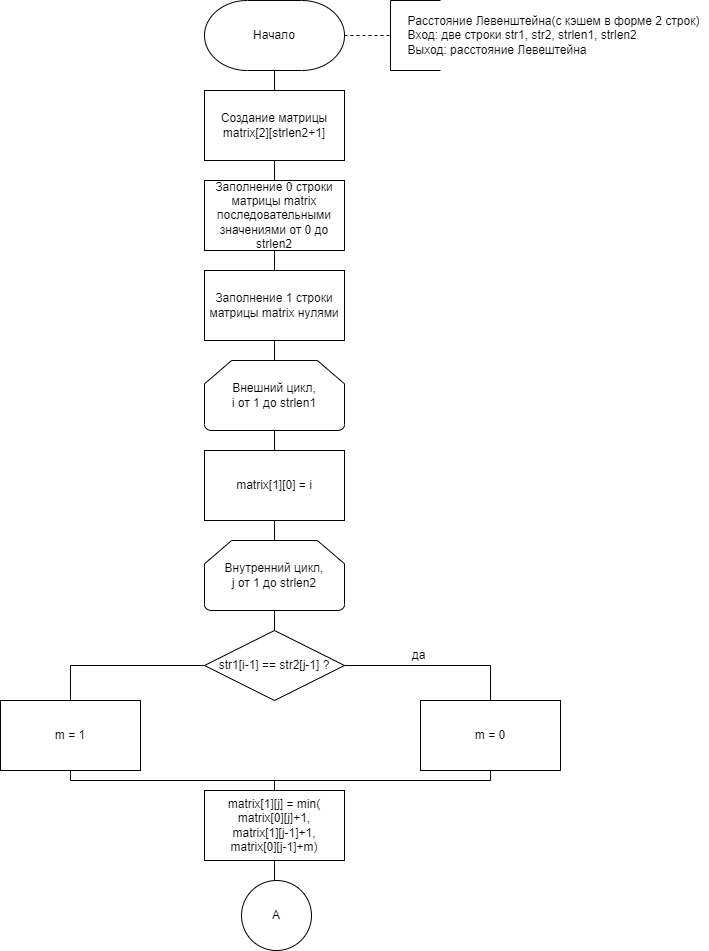
\includegraphics[scale=0.72]{2row1.png}}
\end{figure}
\begin{figure}[H]
\center{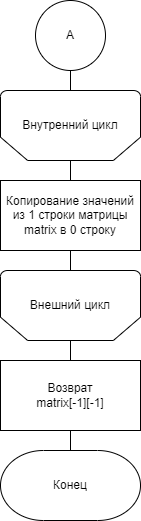
\includegraphics[scale=0.72]{2row2.png}}
\caption*{Рисунок 2.1~--- Расстояние Левенштейна с двухстрочным кэшем}
\end{figure}

\begin{figure}[H]
\center{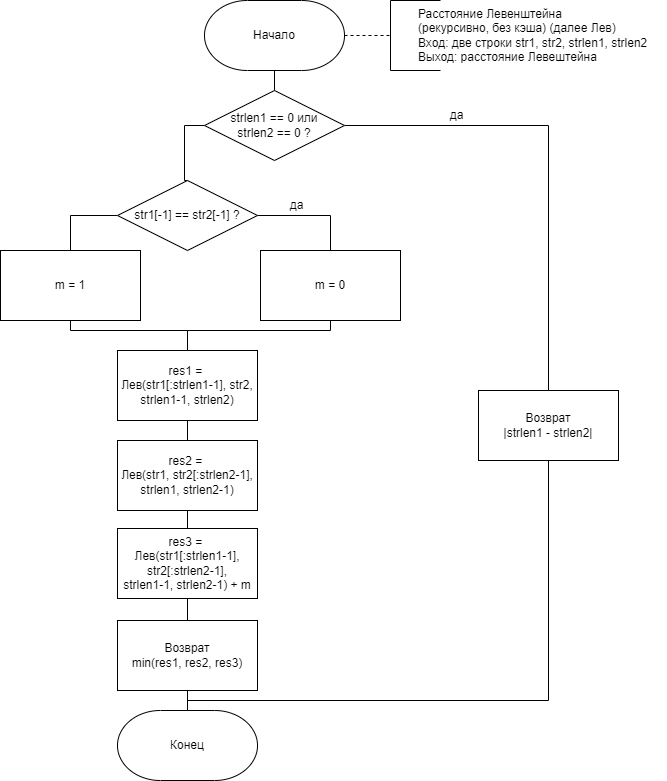
\includegraphics[scale=0.72]{nocache.png}}
\caption*{Рисунок 2.2~--- Расстояние Левенштейна рекурсией без кэша}
\end{figure}

\begin{figure}[H]
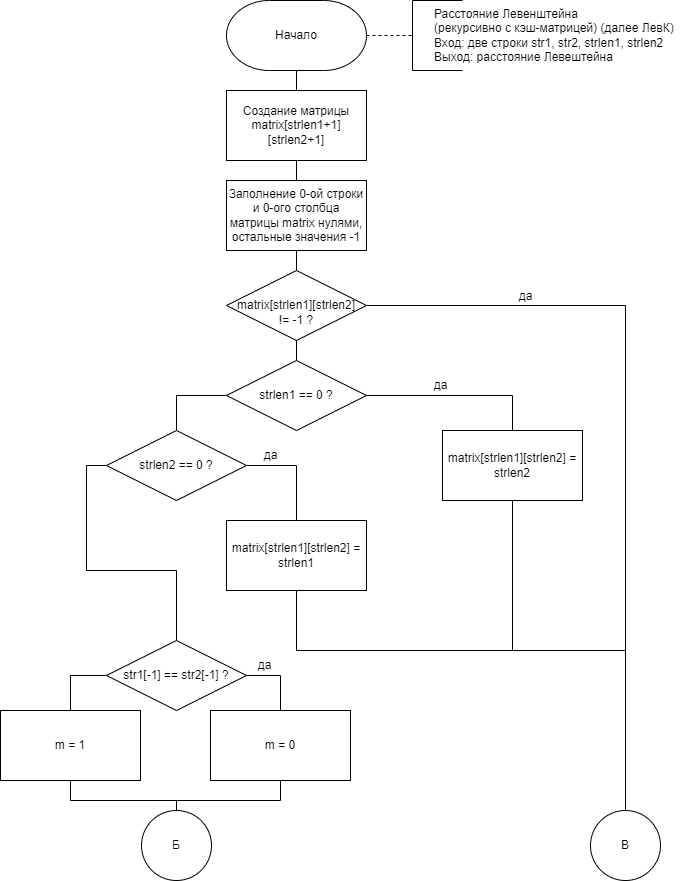
\includegraphics[scale=0.72]{mat1.png}
\end{figure}
\begin{figure}[H]
\center{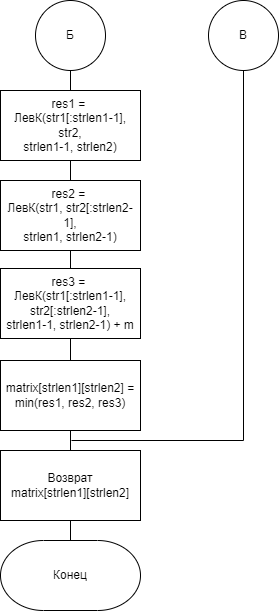
\includegraphics[scale=0.72]{mat2.png}}
\caption*{Рисунок 2.3~--- Расстояние Левенштейна рекурсией с кэш-матрицей}
\end{figure}

\begin{figure}[H]
\center{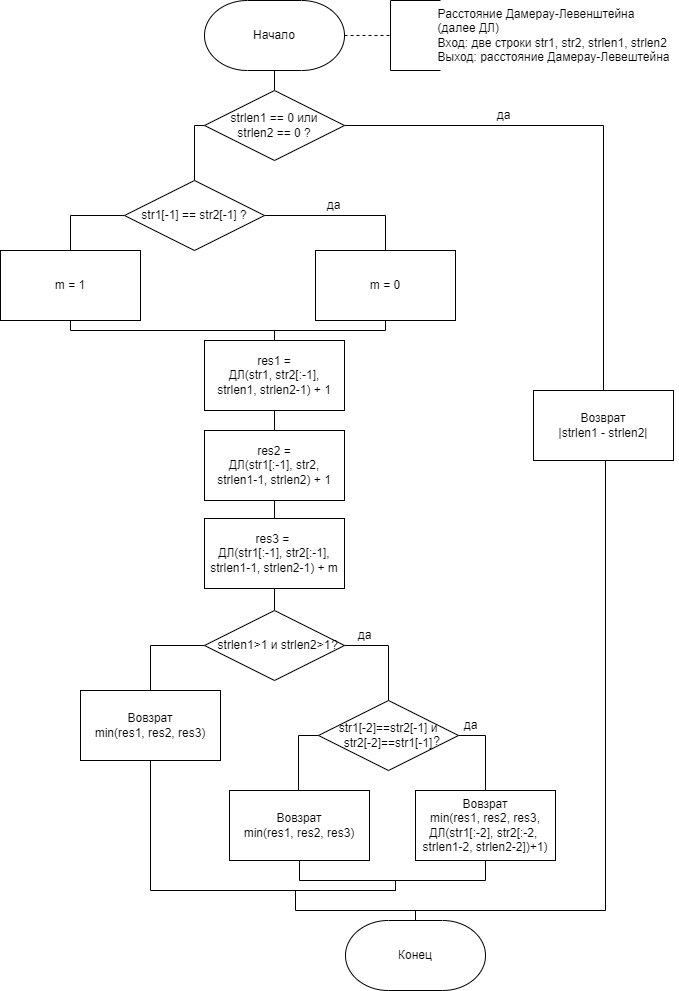
\includegraphics[scale=0.72]{dl.png}}
\caption*{Рисунок 2.4~--- Расстояние Дамерау--Левенштейна}
\end{figure}

\section*{2.2 Вывод по конструкторской части}
\addcontentsline{toc}{section}{2.2 Вывод по конструкторской части}

На основе теоретических данных, полученных из аналитического раздела, были построены схемы алгоритмов нахождения расстояний Левенштейна и Дамерау--Левенштейна.

\chapter*{3 Технологическая часть}
\addcontentsline{toc}{chapter}{3 Технологическая часть}

В данном разделе приведены средства реализации и листинги кода.

\section*{3.1 Требования к ПО}
\addcontentsline{toc}{section}{3.1 Требования к ПО}

К программе предъявляется ряд требований:

\begin{itemize}
	\item на вход ПО получает две строки;
	\item на выходе~--- расстояние Левенштейна (или Дамерау--Левенштейна) для этих строк.
\end{itemize}

\section*{3.2 Средства реализации}
\addcontentsline{toc}{section}{3.2 Средства реализации}

Для реализации ПО был выбран язык программирования \verb|Python| [2]. Это обусловлено знанием возможностей языка, что обеспечит высокую скорость написания программы без потери ее качества. 

В качестве среды разработки была выбрана \verb|Visual Studio Code| [4]. Удобства написания кода и его автодополнения стали ключевыми при выборе.

\section*{3.3 Реализация алгоритмов}
\addcontentsline{toc}{section}{3.3 Реализация алгоритмов}

В листингах 3.1 - 3.4 приведена реализация рассматриваемых алгоритмов.

\newpage
\begin{lstlisting}[title=Листинг 3.1~--- Расстояние Левенштейна с двухстрочным кэшем]
def levTable(str1, str2, strlen1, strlen2):
	matrix = []
	matrix.append([])
	for j in range(strlen2+1):
		matrix[0].append(j)
	if strlen1:
		matrix.append([])
		for j in range(strlen2+1):
			matrix[1].append(0)
	for i in range(1, strlen1+1):
		matrix[1][0] = i
		for j in range(1, strlen2+1):
			matrix[1][j] = min(matrix[0][j] + 1,
					matrix[1][j - 1] + 1,
					matrix[0][j - 1] + lastEqu(str1[:i], str2[:j]))
		matrix[0] = deepcopy(matrix[1])
	return matrix[-1][-1]
\end{lstlisting}

\begin{lstlisting}[title=Листинг 3.2~--- Расстояние Левенштейна рекурсией без кэша]
def levRec(str1, str2, strlen1, strlen2):
	if not str1 or not str2:
		return abs(strlen1 - strlen2)
	res = min(levRec(str1, str2[:-1], strlen1, strlen2-1) + 1,
		levRec(str1[:-1], str2, strlen1-1, strlen2) + 1,
		levRec(str1[:-1], str2[:-1], strlen1-1, strlen2-1) + lastEqu(str1, str2))
	return res
\end{lstlisting}

\newpage
\begin{lstlisting}[title=Листинг 3.3~--- Расстояние Левенштейна рекурсией с кэш-матрицей]
def levRecMatr(str1, str2, strlen1, strlen2):
	matrix = [[i+j if (i == 0 or j == 0) else -1 for j in
	 range(strlen2 + 1)] for i in range(strlen1 + 1)]
	recursion(str1, str2, strlen1, strlen2, matrix)
	return matrix[strlen1][strlen2]

def recursion(str1, str2, i, j, matrix):
	if matrix[i][j] != -1:
		return matrix[i][j]
	if not i or not j:
		return abs(len(str1) - len(str2))
	matrix[i][j] = min(recursion(str1, str2, i - 1, j, matrix) + 1,
		recursion(str1, str2, i, j - 1, matrix) + 1,
		recursion(str1, str2, i - 1, j - 1, matrix) +
		lastEqu(str1[:i], str2[:j]))
	return matrix[i][j]
\end{lstlisting}

\begin{lstlisting}[title=Листинг 3.4~--- Расстояние Дамерау--Левенштейна]
def damlevRec(str1, str2, strlen1, strlen2):
	if not str1 or not str2:
		return abs(strlen1 - strlen2)
	res = min(damlevRec(str1, str2[:-1], strlen1, strlen2-1) + 1,
		damlevRec(str1[:-1], str2, strlen1-1, strlen2) + 1,
		damlevRec(str1[:-1], str2[:-1], strlen1-1, strlen2-1) + lastEqu(str1, str2))
	if (strlen1 > 1 and strlen2 > 1 and str1[-1] == str2[-2] and str1[-2] == str2[-1]):
		res = min(res, damlevRec(str1[:-2], str2[:-2], 
			strlen1-2, strlen2-2) + 1)
	return res
\end{lstlisting}

В листинге (3.5) представлена функция \verb|lastEqu|, использующаяся в алгоритмах поиска расстояний Левенштейна и Дамерау--Левенштейна для определения совпадения последних символов в двух строках.

\newpage
\begin{lstlisting}[title=Листинг 3.5~--- Совпадение последних символов]
def lastEqu(str1, str2):
    if not len(str1) or not len(str2):
        return 1
    return 0 if (str1[-1] == str2[-1]) else 1
\end{lstlisting}

\section*{3.4 Тестовые данные}
\addcontentsline{toc}{section}{3.4 Тестовые данные}

В таблице (3.1) приведены тесты для реализованных функций. Все тесты пройдены успешно.

\begin{table}[H]
	\caption*{Таблица 3.1~--- Тестирование}
		\begin{tabular}[l]{|c|c|c|c|}
			\hline
			Строка1 & Строка2 & Результат & Ожидаемый результат \\\hline
			$\varnothing$ & $\varnothing$  & $0$ & $0$\\\hline
			$\varnothing$  & $data$ & $4$  & $4$\\\hline
			$data$  & $\varnothing$  & $4$  & $4$\\\hline
			$robot$  & $gorod$  & $3$ & $3$\\\hline
			$a$  & $data$  & $3$  & $3$\\\hline
			$data$  & $a$  & $3$  & $3$\\\hline
			$bigdata$  & $ba$  & $5$ & $5$\\\hline
			$ba$  & $bigdata$  & $5$ & $5$\\\hline
			$bigdata$  & $gda$  & $4$ & $4$\\\hline
			$gda$  & $bigdata$  & $4$ & $4$\\\hline
			$ibgcaat$  & $bigdata$  & $5(3^1)$ & $5(3^1)$\\\hline
			$bigdata$  & $ibgcaat$  & $5(3\tablefootnote{расстояние Дамерау--Левенштейна})$ & $5(3^1)$\\\hline
		\end{tabular}
\end{table}

\section*{3.5 Вывод по технологической части}
\addcontentsline{toc}{section}{3.5 Вывод по технологической части}

В данном разделе были разработаны и протестированы реализации алгоритмов нахождения расстояния Левенштейна и Дамерау--Левенштейна.

\chapter*{4 Исследовательская часть}
\addcontentsline{toc}{chapter}{4 Исследовательская часть}

В этом разделе будут исследованы ресурсы, затрачиваемые реализациями алгоритмов, на практических тестах.

\section*{4.1 Технические характеристики}
\addcontentsline{toc}{section}{4.1 Технические характеристики}

Ниже приведены технические характеристики устройства, на котором было проведено тестирование ПО:

\begin{itemize}
	\item Операционная система Windows 10 64-разрядная.
	\item Оперативная память 16 ГБ.
	\item Процессор Intel(R) Core(TM) i5-4690 @ 3.50ГГц.
\end{itemize}

\section*{4.2 Время выполнения реализаций алгоритмов}
\addcontentsline{toc}{section}{4.2 Время выполнения реализаций алгоритмов}

Время выполнения алгоритмов замерялось с помощью специальной функции \verb|process_time()| [3] из модуля \verb|time|, которая возвращает значение в долях секунды процессорного времени текущего процесса. Контрольная точка возвращаемого значения не определена, поэтому допустима только разница между результатами последовательных вызовов.

В таблице 4.1 и на графиках 4.1 - 4.2 показаны результаты замеров. Все значения времени выполнения отображены в секундах.

\newpage
\begin{table} [H]
	\caption*{Таблица 4.1~--- Зависимость времени выполнения реализаций алгоритмов от длины строк}
	\begin{tabular}[l]{|c c c c c|}
		\hline
		Длина строк & LevCache\tablefootnote[1]{расстояние Левенштейна с кэшем в форме 2 строк} & LevRec\tablefootnote{расстояние Левенштейна рекурсией без кэша} & LevRecCache\tablefootnote{расстояние Левенштейна рекурсией с кэш-матрицей} & Dam--Lev\tablefootnote{расстояние Дамерау--Левенштейна}  \\

		5 & 0.00002837 & 0.00185848 & 0.00002587 & 0.00166622 \\\hline 

		6 & 0.00003048 & 0.00767277 & 0.00002683 & 0.00806983 \\\hline 

		7 & 0.00003959 & 0.04125901 & 0.00003292 & 0.04837457 \\\hline 

		8 & 0.00008390 & 0.28312333 & 0.00007510 & 0.28398161 \\\hline 

		9 & 0.00010394 & 1.55095931 & 0.00009646 & 1.47087310 \\\hline 

		10 & 0.00013424 & 7.02560350 & 0.00012200 & 8.41714851 \\\hline
	\end{tabular}
\end{table}

\begin{figure}[H]
\caption*{График 4.1~--- Зависимость времени выполнения от длины строк (алгоритмы нахождения расстояния Левенштейна рекурсивно с кэш-матрицей и итеративно с кэшем в форме 2 строк)}
\begin{center}
\begin{tikzpicture}
\begin{axis}[
	xlabel = {$Длина\text{ }строк$},
	ylabel = {$Время, сек$},
	legend pos = north west,
	height = 0.4\paperheight, 
	width = 0.7\paperwidth,
	xmin = 4,
	xmax = 11
]
\legend{ 
	$\text{Левенштейн(рекурсивно, кэш-матрица)}$, 
	$Левенштейн(двухстрочный\text{ }кэш)$
};
\addplot coordinates {
	(5,0.00002587) (6,0.00002683) (7,0.00003292) (8,0.00007510) (9,0.00009646) (10,.00012200)
};
\addplot coordinates {
	(5,0.00002837) (6,0.00003048) (7,0.00003959) (8,0.00008390) (9,0.00010394) (10,.00013424)
};
\end{axis}
\end{tikzpicture}
\end{center}
\end{figure}

\begin{figure}[H]
\caption*{График 4.2~--- Зависимость времени выполнения от длины строк (алгоритмы нахождения расстояния Левенштейна рекурсивно без кэша и Дамерау--Левенштейна)}
\begin{center}
\begin{tikzpicture}
\begin{axis}[
	xlabel = {$Длина\text{ }строк$},
	ylabel = {$Время, сек$},
	legend pos = north west,
	height = 0.4\paperheight, 
	width = 0.7\paperwidth,
	xmin = 4,
	xmax = 11
]
\legend{ 
	$Левенштейн(рекурсивно)$, 
	$Дамерау\text{--}Левенштейн$
};
\addplot coordinates {
	(5,0.00185848) (6,0.00767277) (7,0.04125901) (8,0.28312333) (9,1.55095931) (10,7.02560350)
};
\addplot coordinates {
	(5,0.02560350) (6,0.00806983) (7,0.04837457) (8,0.28398161) (9,1.47087310) (10,8.41714851)
};
\end{axis}
\end{tikzpicture}
\end{center}
\end{figure}

\section*{4.3 Используемая память}
\addcontentsline{toc}{section}{4.3 Используемая память}

Пусть $str1$, $str2$~--- строки, $strlen1$~--- длина строки $str1$, $strlen2$~--- длина строки $str2$, $sizeof$~--- операция получения размера типа данных на конкретной машине. Тогда, рассчитаем объем используемой памяти для каждого алгоритма.

\textbf{Алгоритм Левенштейна с кэшем в виде двух строк}
\begin{itemize}
	\item две целочисленные переменные для хранения длин строк $2sizeof(int) $;
	\item память для хранения строк $(strlen1 + strlen2) \cdot sizeof(char)$;
	\item память для хранения кэш-матрицы $(strlen2 + 1) \cdot 2sizeof(int)$;
	\item память для хранения 2 целочисленных вспомогательных переменных $2 \cdot sizeof(int)$.
\end{itemize}
Суммарная память представлена в формуле (4.1). $$(strlen1 + strlen2) \cdot sizeof(char) + (strlen2 + 3) \cdot 2sizeof(int) \eqno (4.1)$$\\

\textbf{Рекурсивный алгоритм Левенштейна}

Максимальная глубина стека вызовов при рекурсивной реализации равна сумме длин входящих строк. Для каждого вызова:

\begin{itemize}
	\item две целочисленные переменные для хранения длин строк $2sizeof(int)$;
	\item память для хранения строк $(strlen1 + strlen2) \cdot sizeof(char)$;
	\item память для хранения одной целочисленной вспомогательной переменной $sizeof(int)$;
	\item память для хранения адреса возврата $sizeof(int*)$.
\end{itemize}
Суммарная память представлена в формуле (4.2). $$(strlen1 + strlen2) \cdot$$$$\cdot ((strlen1 + strlen2) \cdot sizeof(char) + 3sizeof(int) + sizeof(int*)) \eqno (4.2)$$\\

\textbf{Рекурсивный алгоритм Левенштейна с кэш-матрицей}

Память для хранения кэш-матрицы $(strlen1 + 1)(strlen2 + 1) \cdot sizeof(int)$.

Для каждого вызова:
\begin{itemize}
	\item две целочисленные переменные для хранения длин строк $2sizeof(int)$;
	\item память для хранения строк$(strlen1 + strlen2) \cdot sizeof(char)$;
	\item память для хранения 2 целочисленных вспомогательных переменных $2sizeof(int)$;
	\item память для хранения ссылки на матрицу $sizeof(int*)$;
	\item память для хранения адреса возврата $sizeof(int*)$.
\end{itemize}
Суммарная память представлена в формуле (4.3). $$(strlen1 + 1) \cdot (strlen2 + 1) \cdot sizeof(int) + (strlen1 + strlen2) \cdot$$$$\cdot ((strlen1 + strlen2) \cdot sizeof(char) + 4sizeof(int) + 2sizeof(int*)) \eqno (4.3)$$\\

\newpage
\textbf{Алгоритм Дамерау--Левенштейна}

Аналогичен рекурсивному алгоритму Левенштейна без использования кэша, однако используется дополнительная целочисленная переменная.
	Суммарная память представлена в формуле (4.4). $$(strlen1 + strlen2) \cdot$$$$\cdot ((strlen1 + strlen2) \cdot sizeof(char) + 4sizeof(int) + sizeof(int*)) \eqno (4.4)$$
	
\section*{4.4 Вывод по исследовательской части}
\addcontentsline{toc}{section}{4.4 Вывод по исследовательской части}

Проведены замеры времени выполнения реализаций алгоритмов и оценено количество затрачиваемой памяти.

По результатам самый быстрый алгоритм~--- алгоритм нахождения расстояния Левенштейна рекурсией с использованием кэш-матрицы, при этом является самым затратным с точки зрения памяти, в среднем этот алгоритм затрачивает памяти больше на размер кэш-матрицы. Значит с увеличением длин строк, он будет требовать все больше памяти.

Самым медленным алгоритмом, явно на больших длинах строк, является алгоритм нахождения расстояния Дамерау--Левенштейна.

Алгоритм нахождения расстояния Левенштейна с использованием двухстрочного кэша требует меньше всего памяти за счет отсутствия рекурсивных вызовов.

\chapter*{Заключение}
\addcontentsline{toc}{chapter}{Заключение}

В ходе проделанной работы была достигнута поставленная цель и решены следующие задачи:

\begin{itemize}
	\item были изучены алгоритмы нахождения расстояний Левенштейна и\newline Дамерау--Левенштейна;
	\item эти алгоритмы были реализованы и успешно протестированы;
	\item был проведён сравнительный анализ алгоритмов по времени работы и количеству затрачиваемой памяти.
\end{itemize}

Выбор конкретного алгоритма нахождения расстояния будет зависеть от исходных данных и поставленной задачи. Для достижения наивысшей скорости работы, при этом потери большого количества памяти следует выбрать алгоритм нахождения расстояния Левенштейна рекурсией с использованием кэш-матрицы. Самым сбалансированным вариантом является итеративный алгоритм с использованием кэша в форме двух строк.

\chapter*{Литература}
\addcontentsline{toc}{chapter}{Литература}

[1] Левенштейн В.И. Двоичные коды с исправлением выпадений, вставок и замещений символов. Доклады АН СССР, 1965. Т. 163. С. 845-848. \\

[2] Python [Электронный ресурс]. Режим доступа: https://python.org. Дата обращения: 10.10.2021.\\

[3] Модуль time [Электронный ресурс]. Режим доступа: \newline https://docs.python.org/3/library/time.html. Дата обращения: 10.10.2021.\\

[4] Visual Studio Code - Code Editing [Электронный ресурс]. Режим доступа: https://code.visualstudio.com. Дата обращения: 10.10.2021.

\end{document}